\chapter{Trabalhos Relacionados}
\label{cap:trabalhos-relacionados}

Nesta seção, estão descritas algumas ferramentas de visualização de algoritmos de análise sintática, suas funcionalidades e limitações.

\section{\textit{Project-based Learning}}

No trabalho de \textcite{larapbl} foi utilizada a técnica de ensino \gls{pbl} na disciplina de compiladores. O trabalho explica como o projeto criado é mais adequado para uso da técnica \gls{pbl} do que os projetos comumente usados na disciplina de compiladores e como os alunos responderam a utilização do projeto. Por fim o trabalho conclui que o projeto criado foi capaz de aumanetar a motivação dos alunos mais do que as outras tecnicas de ensino usadas na disciplina.

\section{\textit{Automatic Question Generation
and Intelligent Assessment of Grammars' Parsing}}
\textcite{munozquestions} criaram uma aplicação de geração automática de questões para o ensino de compiladores. As funcionalidades da aplicação incluem a geração automática de gramáticas livres de contexto, geração de questões e interface apropriada para resposta, correção automática e disponilização de \textit{feedback} sobre erros cometidos.

\section{\textit{Parser Generator Web Tools}}
\label{sec:trabalho-relacionado-a}

Essa ferramenta desenvolvida por \textcite{Parser-2024-04-12} é uma aplicação \textit{web} que oferece a visualização de três algoritmos, LL(1), SLR e CLR. Através da caixa de entrada é informada uma gramática e partir dela são geradas automaticamente a tabela dos conjuntos \textit{first} e \textit{follow} como mostra a Figura \ref{fig:sets}. Também são gerados um autômato dos estados do analisador sintático e a tabela de transição de estados como mostra a Figura \ref{fig:tableandautomata}. Além disso é disponibilizado para \textit{download} o código com a declaração das estruturas usadas no algoritmo e a atribuição manual dos dados gerados pelo algoritmo.

\begin{figure}[ht]
    \captionsetup{width=16cm}
    \Caption{\label{fig:sets} Imagem da ferramenta de \textit{Parser Generator Web Tools}}
    \tcbox[left=0cm, right=0cm, top=0cm, bottom=0cm,center]{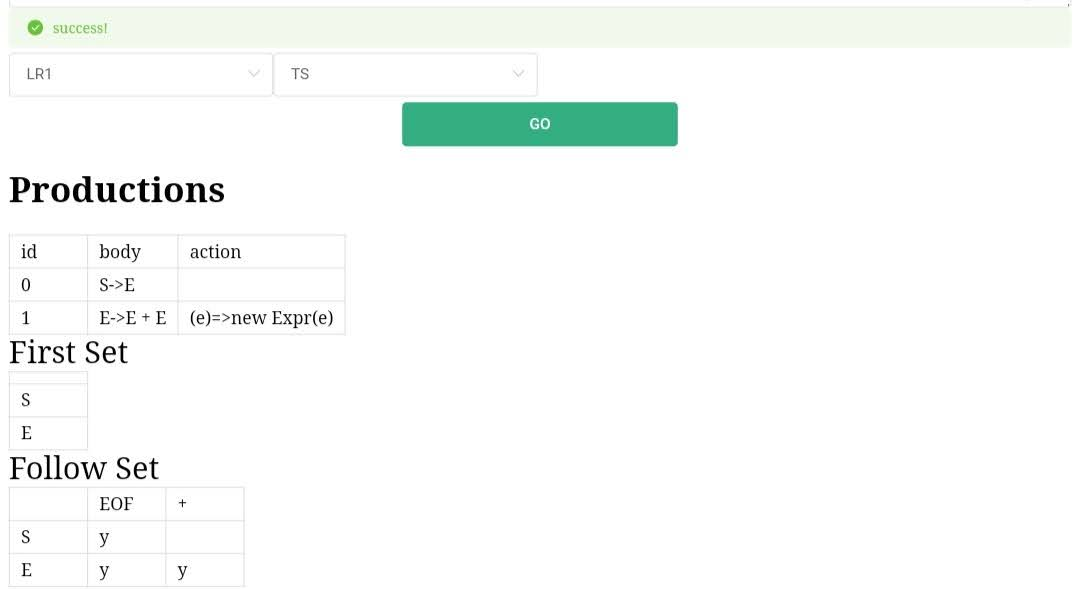
\includegraphics[width=15.6cm]{figuras/lightparsers2.jpg
    }}{\Fonte{\textcite{Parser-2024-04-12}.}}
\end{figure}

\section{LR(1) \textit{Parser Generator}}
Feita especificamente para o algoritmo CLR a ferramenta \textit{web} criada por \textcite{LR-2024-04-12} gera o conjunto de \textit{first} mostrado na Figura \ref{fig:firstandcanonical}, o conjunto de itens canônicos mostrado na Figura \ref{fig:firstandcanonical} e a tabela de transição de estados mostrada na Figura \ref{fig:tableandparse}. A ferramenta também disponibiliza o passo a passo da análise de uma \textit{string} junto com uma árvore sintática representada por contêineres contidos um dentro do outro como mostra a Figura \ref{fig:tableandparse}.

\begin{figure}[ht]
    \captionsetup{width=16cm}
    \Caption{\label{fig:tableandautomata}Imagem da ferramenta de \textit{Parser Generator Web Tools}}
    \tcbox[left=0cm, right=0cm, top=0cm, bottom=0cm,center]{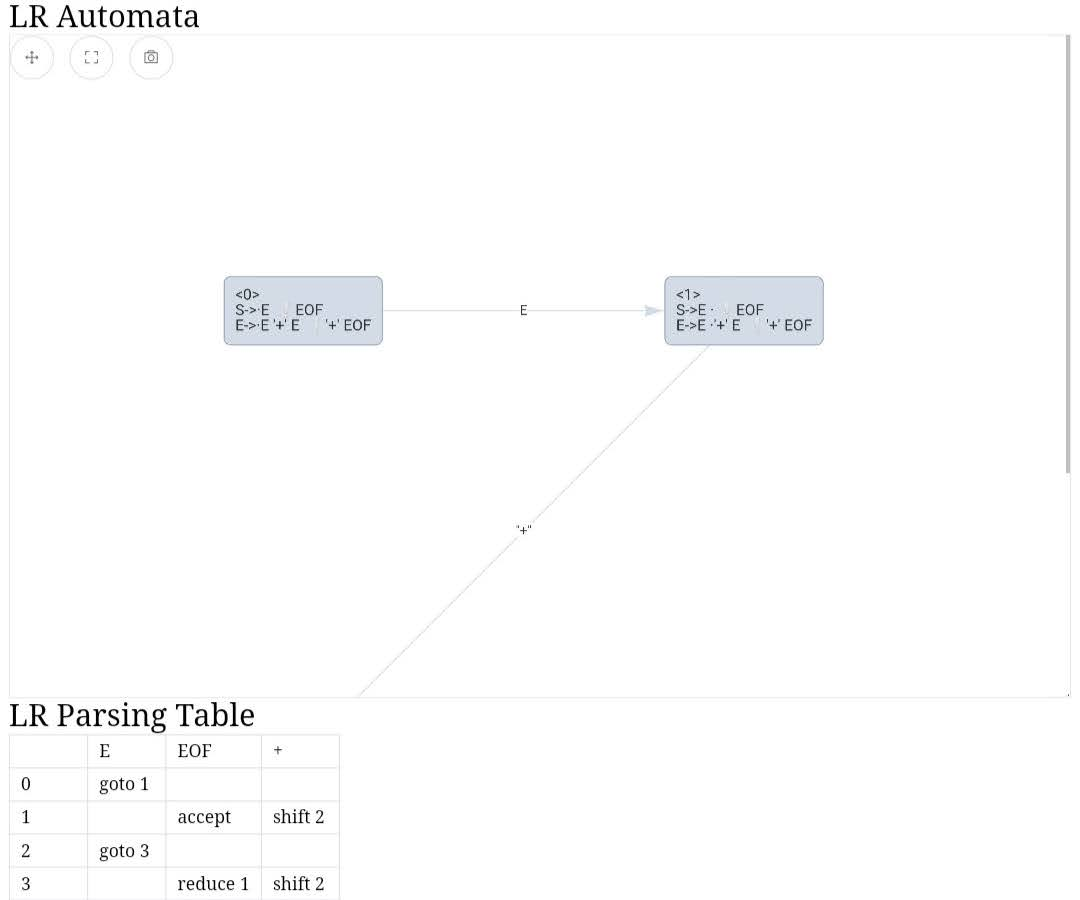
\includegraphics[width=15.6cm]{figuras/lightparsers.jpg}}
    {\Fonte{\textcite{Parser-2024-04-12}.}}
\end{figure}

\begin{figure}[ht]
    \captionsetup{width=16cm}
    \Caption{\label{fig:firstandcanonical}Imagem da ferramenta de LR(1) \textit{Parser Generator}}
    \tcbox[left=0cm, right=0cm, top=0cm, bottom=0cm,center]{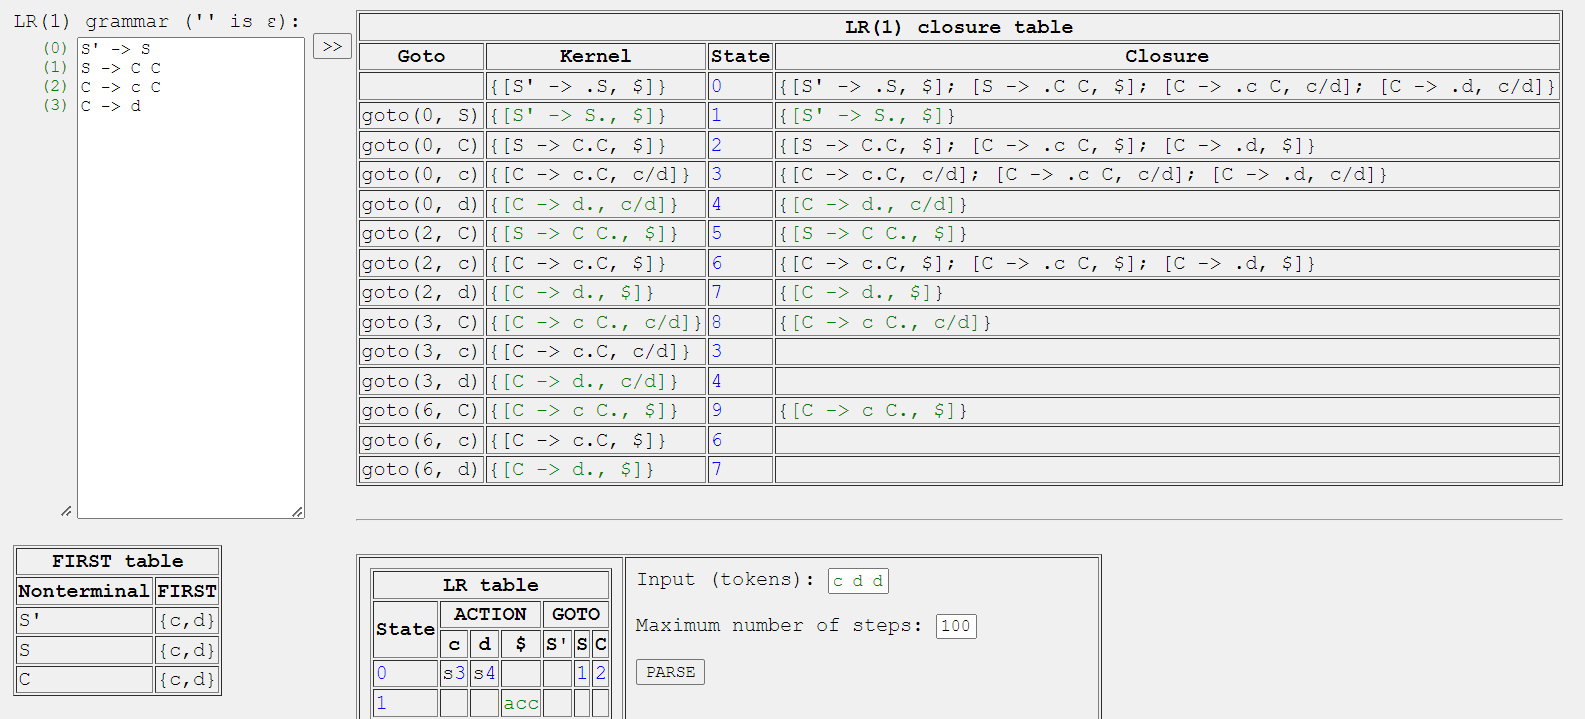
\includegraphics[width=15.6cm]{figuras/lrparser2.png}}{
    \Fonte{\textcite{LR-2024-04-12}.}}
\end{figure}

\begin{figure}[ht]
    \captionsetup{width=16cm}
    \Caption{\label{fig:tableandparse}Imagem da ferramenta de LR(1) \textit{Parser Generator}}
    \tcbox[left=0cm, right=0cm, top=0cm, bottom=0cm,center]{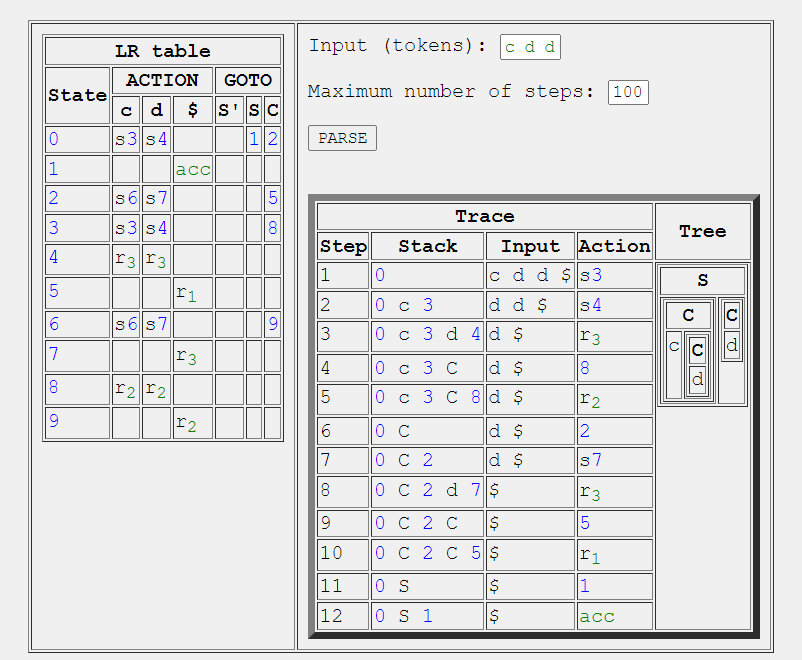
\includegraphics[width=15.6cm]{figuras/lrparser.png}}{
    \Fonte{\textcite{LR-2024-04-12}.}}
\end{figure}
%\FloatBarrier

\section{PAVT}
No trabalho de \textcite{sangal2018pavt} foi criada a ferramenta PAVT (\textit{Parsing Algorithms Visualization Tool}) para visualização de seis algoritmos de análise sintática. A ferramenta apresenta uma caixa de entrada para informar a gramática a opção de importar uma gramática através de um arquivo, uma caixa de entrada para as \textit{string} a serem analisadas e uma breve descrição dos algoritmos disponíveis. Todos os elementos da ferramenta podem ser vistos na Figura \ref{fig:pavt}. Apesar da ferramenta oferecer a visualização dos algoritmos, essa visualização é realizada apenas pela leitura de um arquivo de texto gerado pela ferramenta, além de não mostrar instruções de como chegar ao resultado descrito no arquivo de texto. O \textit{software} também está apenas disponível em versão \textit{desktop} para o sistema operacional \textit{Windows}.

\section{JFLAP}
JFLAP (\textit{Java Formal Languages and Automata Package}) é uma ferramenta \textit{desktop} criada por \textcite{jflap} que pode ser usada para visualização dos algoritmos LL(1), SLR e de força bruta. Como mostra a Figura \ref{fig:jflap}, a ferramenta apresenta os conjuntos \textit{first} e \textit{follow}, o autômato dos estados do analisador sintático e a tabela de ações. O processo de \textit{parsing} também é disponibilizado assim como a árvore sintática. Apesar de a visualização ser feita por meio de uma interface gráfica, assim como na ferramenta citada na seção anterior, JFLAP não dá instruções de como chegar nos resultados mostrados.

\section{Considerações}
Apesar de já existirem ferramentas de visualização de \textit{parsers}, algumas desvantagens ainda precisam ser consideradas. Uma limitação é que o conteúdo não tem muita interatividade, a ferramenta PAVT, por exemplo, apresenta apenas em um arquivo de texto. Isso pode dificultar a compreensão dos conceitos. A ferramenta \textit{Parser Generator Web Tools} não oferece a visualização da árvore sintática que é um elemento fundamental para entender a estrutura da análise sintática. Outro ponto fraco é a falta de detalhamento do passo a passo dos algoritmos, o que impede que os estudantes acompanhem o funcionamento interno dos processos de análise. A variedade de algoritmos de análise sintática disponíveis nas ferramentas pode ser limitada, restringindo a exposição dos alunos a diferentes abordagens e técnicas. Por fim, nenhuma das ferramentas apresenta uma versão \textit{mobile}. Essas lacunas representam oportunidades de melhoria para que as ferramentas de visualização de \textit{parsers} se tornem ainda mais eficazes no apoio ao ensino e aprendizagem de análise sintática. No Quadro \ref{qua:comparativo} pode-se ver o resumo do comparativo dos trabalhos citados anteriormente.

\setlength{\abovecaptionskip}{10pt plus 0pt minus 0pt}
\setlength{\belowcaptionskip}{5pt plus 0pt minus 0pt}
\begin{table}[h]
\centering\setlength{\extrarowheight}{2pt}
\captionsetup{width={\textwidth}}
\captionof{quadro}{Comparativo de trabalhos relacionados}\label{qua:comparativo}
\resizebox{\textwidth}{!}{\begin{NiceTabular}{l*{7}{c}}[corners,hvlines]
\CodeBefore
  \rowcolor{gray!15}{1-2}
\Body
\Block{2-1}{Trabalho}&\Block{1-3}{Algoritmos}&&&\Block{1-3}{Plataformas}&&&\Block{2-1}{Integração com Moodle}\\

&LL(1)&SLR&CLR&Mobile&Desktop&Web\\
\textcite{jflap}                   &x& & & & & \\
\textcite{LR-2024-04-12}   & &x&x& & & \\
\textcite{Parser-2024-04-12}               & & &x&x&x& \\
\textcite{pavt}             & & &x&x&x& \\
Este trabalho &x&x&x&x&x&x&x \\
\end{NiceTabular}}
{\Fonte{fornecido pelo autor}}
\end{table}

\begin{figure}[h]
    \captionsetup{width=16cm}
    \Caption{\label{fig:pavt}Imagem da ferramenta PAVT}
    \tcbox[left=0cm, right=0cm, top=0cm, bottom=0cm,center]{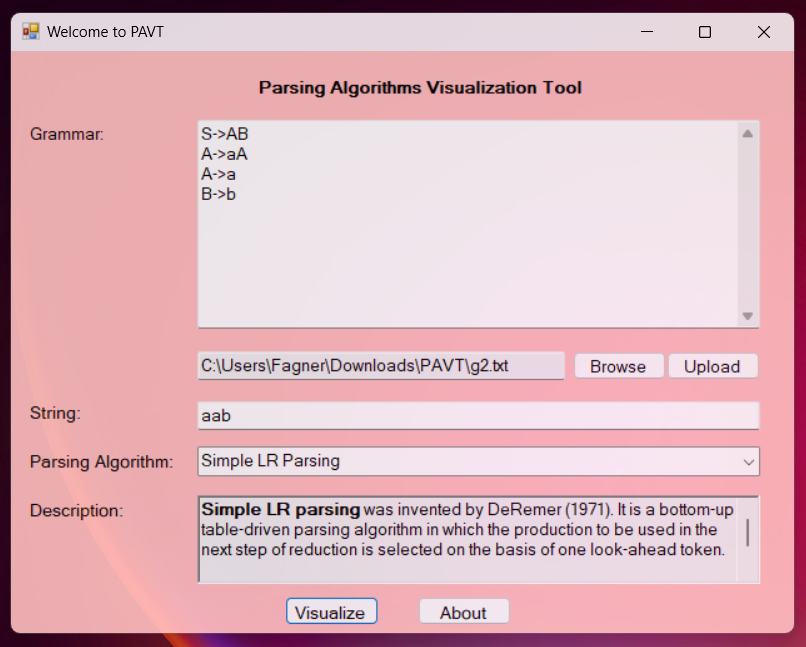
\includegraphics[width=15.6cm, height=10.0cm]{figuras/pavt.png}}{
    \Fonte{\textcite{pavt}.}}
\end{figure}
\begin{figure}[h]
    \captionsetup{width=16cm}
    \Caption{\label{fig:jflap}Imagem da ferramenta JFLAP}
    \tcbox[left=0cm, right=0cm, top=0cm, bottom=0cm,center]{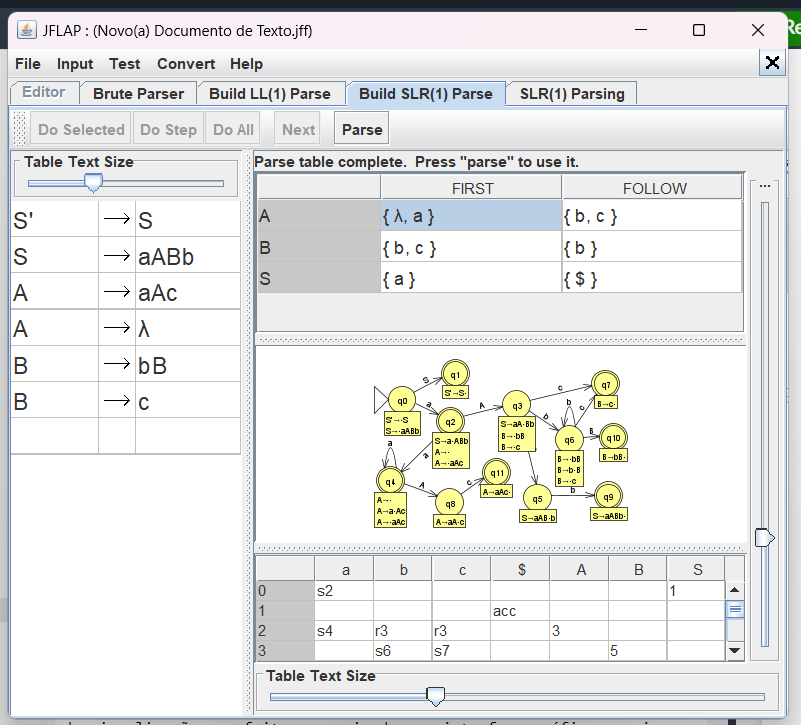
\includegraphics[width=15.6cm, height=7.95cm]{figuras/jflap.png}}{
    \Fonte{\textcite{jflap}.}}
\end{figure}

\begin{figure}[t!]
    \captionsetup{width=16cm}
    \Caption{\label{fig:jflapparse}Imagem da ferramenta JFLAP}
    \tcbox[left=0cm, right=0cm, top=0cm, bottom=0cm,center]{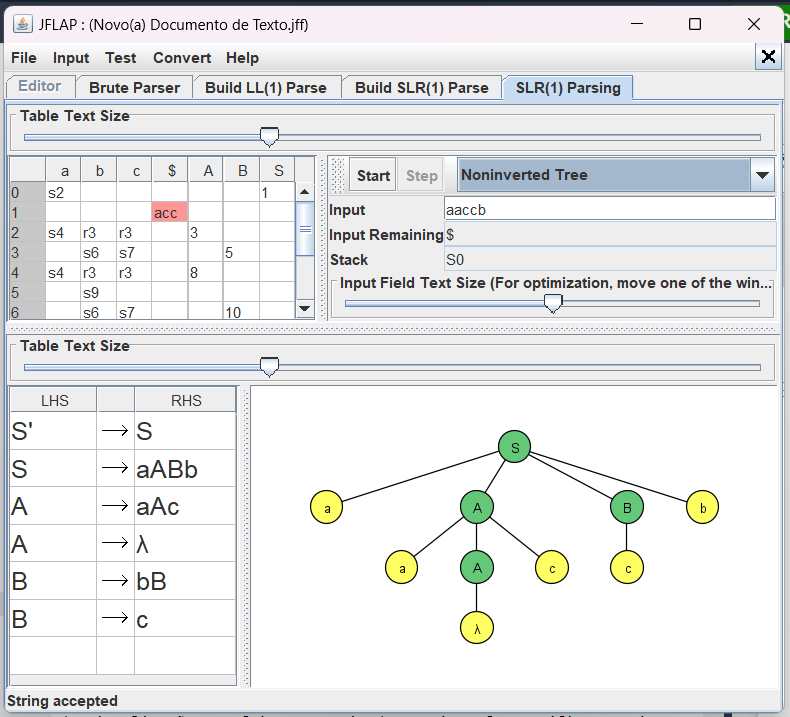
\includegraphics[width=15.6cm, height=7.85cm]{figuras/jflapparse.png}}{
    \Fonte{\textcite{jflap}.}}
\end{figure}
%\FloatBarrier
